%-------------------------------------------------------------------------------
%                            BAB II
%               TINJAUAN PUSTAKA DAN DASAR TEORI
%-------------------------------------------------------------------------------
%\fancyhf{}
% \fancyfoot[C]{\thepage}
\chapter{TINJAUAN KEPUSTAKAAN}
% \thispagestyle{plain} % Halaman pertama bab menggunakan gaya plain



\par Untuk mendukung penelitian ini, maka dalam bab ini akan dikemukakan beberapa rumusan teori pendukung yang dikutip dari berbagai referensi baik dalam bentuk buku, artikel, maupun tulisan karya ilmiah lainnya, termasuk hasil penelitian sebelumnya yang ada kaitannya dengan penelitian yang dilakukan.

% Mengatur format untuk bagian (section)

\section{Machine Learning}
\par \textit{Machine Learning} adalah cabang dari ilmu kecerdasan buatan (AI) yang berfokus pada pengembangan sistem yang dapat belajar dari data. Salah satu jenisnya adalah \textit{Supervised Learning}, di mana model dilatih menggunakan data yang sudah dilabeli \citep{johnstonsign2007}.  \ref{fig:machine_learning}.

% contoh penggungaan gambar dengan subfigure
\begin{figure}[H] 
    \centering \begin{subfigure}[b]{0.44\textwidth} 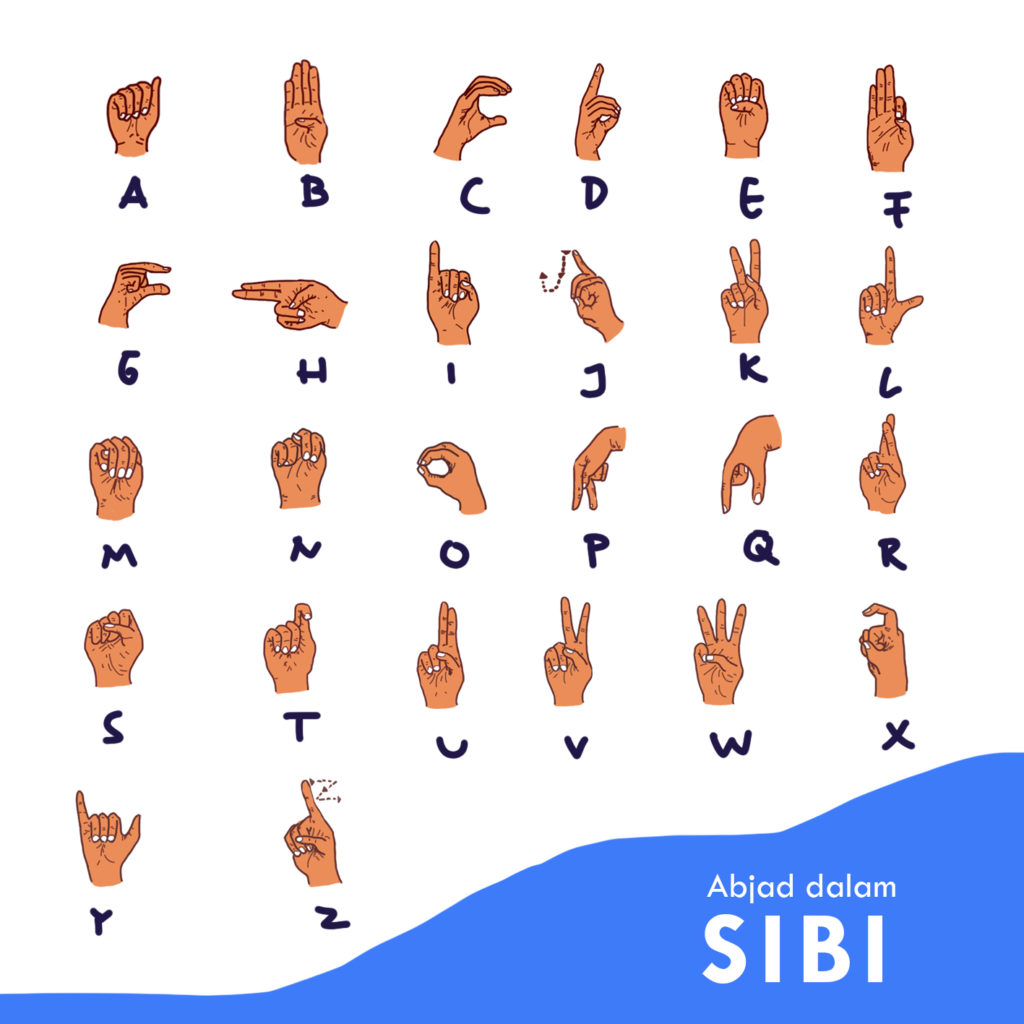
\includegraphics[width=\textwidth]{image/bab2/SIBI.jpg} \caption{} 
\label{fig:machine} 
\end{subfigure} 
\hfill 
    \begin{subfigure}[b]{0.44\textwidth} 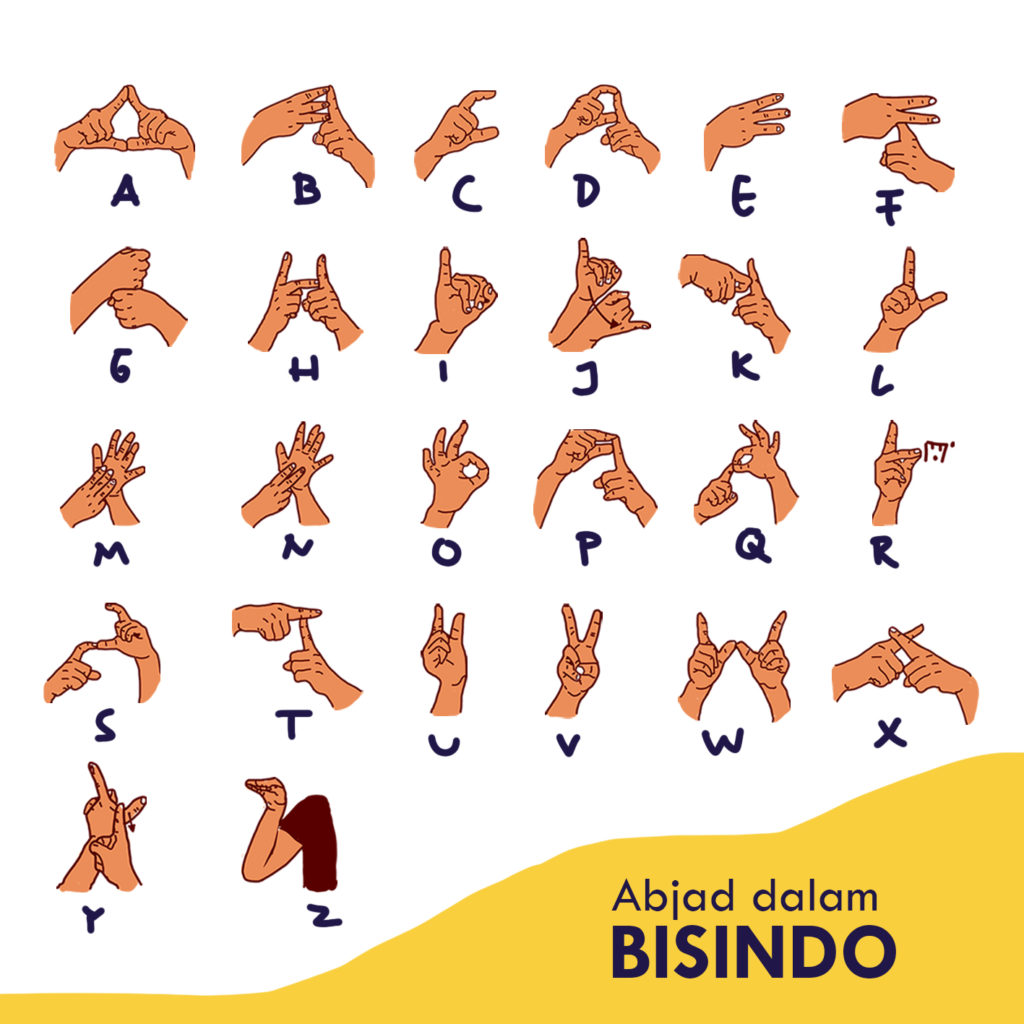
\includegraphics[width=\textwidth]{image/bab2/BISINDO.JPG} \caption{} 
    \label{fig:learning} 
\end{subfigure} 
\caption{Machine Learning\citep{mzakyrakhmat2024Bisindo}} 
\label{fig:machine_learning} 
\end{figure}

\subsection{E-Learning dan Analisis Pengguna}
\par E-learning adalah sistem pembelajaran berbasis teknologi informasi yang memungkinkan proses belajar secara online. Analisis pengguna menjadi penting untuk mengetahui pola penggunaan dan performa sistem \citep{setiawan2023pemanfaatan}. E-learning memiliki beberapa karakteristik yang terbentuk dari sistem pelaksanaannya. Karakteristik yang pertama, ketika kita merujuk pada bahasa secara harfiah atau segi epistemologi dari e-learning sendiri yang berarti pembelajaran secara online atau elektronik, maka dapat dikatakan karakterisik e-learning adalah memanfaatkan media digital dan jasa teknologi elektronik \citep{nadywebsite}.

\section{\textit{Computer Vision}}
\par \textit{Computer vision} adalah cabang ilmu komputer yang berfokus pada pengembangan algoritme dan sistem untuk memahami serta menganalisis informasi dari data visual, seperti gambar dan video. Dengan memadukan prinsip-prinsip matematika, statistik, dan kecerdasan buatan, \textit{computer vision} bertujuan untuk mereplikasi kemampuan manusia dalam mengenali dan menafsirkan dunia visual. Bidang ini membentuk dasar bagi berbagai inovasi modern dalam teknologi analisis visual \citep{szeliski2022computer}.

\section{\textit{Deep Learning}}
\par \textit{Deep Learning} adalah cabang pembelajaran mesin yang menggunakan arsitektur jaringan saraf berlapis-lapis (\textit{deep neural networks}) untuk mempelajari representasi data secara hierarkis, dengan lapisan yang lebih dalam mampu menangkap pola atau fitur yang lebih kompleks \citep{Goodfellow-et-al-2016}. 

\section{K-Nearest Neighbors}
\par Algoritma K-Nearest Neighbors merupakan salah satu metode supervised learning yang digunakan untuk klasifikasi dan regresi \cite{bishop2006pattern}. K-Nearest Neighbors (KNN) adalah algoritma non-parametrik yang tidak melakukan pelatihan eksplisit, namun menyimpan seluruh dataset untuk proses inferensi. Jarak antar data dihitung menggunakan rumus Euclidean Distance. Persamaan KNN dapat dilihat pada \ref{eq:knn_distance}
\vspace{-1em}
\begin{equation}
    d(x,y) = \sqrt{\sum_{i=1}^{n}(x_i - y_i)^2}
    \label{eq:knn_distance}
\end{equation}

\vspace{-1em}
\hspace{0.2cm}dengan
\vspace{-0.8em}
\begin{align*}
    x_i &: \text{fitur ke-}i\text{ dari dua data posisi $x_i$ } \\
    y_i &: \text{fitur ke-}i\text{ dari dua data posisi $y_i$} \\
    n        &: \text{jumlah total fitur}
\end{align*}

\section{\textit{Transfer Learning}}
\par \textit{Transfer learning} adalah pendekatan pembelajaran mesin yang memanfaatkan pengetahuan dari tugas sebelumnya untuk meningkatkan kinerja pada tugas baru yang terkait. Dengan mentransfer informasi dari domain sumber ke domain target, metode ini mengurangi kebutuhan data besar, mempercepat pelatihan, dan meningkatkan generalisasi model \citep{zhuang2020comprehensive}. Ilustrasi teknik  \textit{transfer learning}  dapat dilihat pada gambar \ref{transfer_learning}.

\begin{figure}[H]
\centering
{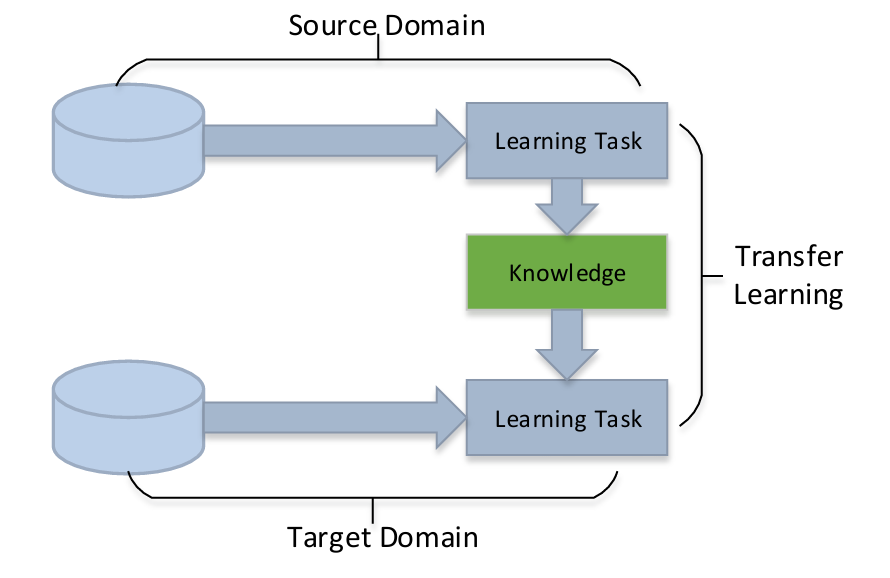
\includegraphics [width = 7cm, height= 4.2cm]{image/bab2/transfer-learning.png}}
\caption{Contoh \textit{transfer learning} \citep{tan2018survey}}
\label{transfer_learning}
\end{figure}


\section{Metrik Evaluasi}
\par Metrik evaluasi adalah alat yang digunakan untuk evaluasi model klasifikasi berdasarkan prediksi yang dihasilkan dibandingkan dengan label kebenaran. Metrik ini menilai secara keseluruhan dan per kelas .  \citep{han2011data}.

\subsection{\textit{Confusion Matrix}}
\par \textit{Confusion matrix} adalah representasi tabel yang merangkum hasil prediksi model klasifikasi, di mana baris merepresentasikan kelas sebenarnya dan kolom merepresentasikan kelas hasil prediksi \citep{han2011data}. Ada empat elemen yang digunakan untuk memahami evaluasi dari \textit{Confusion matrix} yaitu:
\begin{itemize}
    \item TP (\textit{True Positive}): jumlah prediksi yang benar untuk suatu kelas tertentu.
    \item TN (\textit{True Negative}): jumlah prediksi benar untuk kelas lain selain kelas yang sedang dianalisis.
    \item FP (\textit{False Positive}): jumlah prediksi salah di mana kelas lain diklasifikasikan sebagai kelas tersebut.
    \item FN (\textit{False Negative}): jumlah prediksi salah di mana kelas tersebut diklasifikasikan sebagai kelas lain.
\end{itemize}

\subsection{Akurasi}
\par Akurasi mengukur proporsi prediksi yang benar terhadap keseluruhan prediksi. Rumus akurasi diberikan pada persamaan \ref{eq:akurasi} \citep{han2011data}.
\begin{equation}
\text{Akurasi} = \frac{TP + TN}{TP + TN + FP + FN}
\label{eq:akurasi}
\end{equation}


\subsection{\textit{Precision}}
\par \textit{Precision} adalah proporsi dari semua prediksi positif yang benar-benar positif. Presisi penting dalam situasi di mana kesalahan positif palsu (\textit{False Positives}) harus diminimalkan. Rumusnya diberikan pada persamaan \ref{eq:presisi} \citep{powers2020evaluation}.
\begin{equation}
\text{Presisi} = \frac{TP}{TP + FP}
\label{eq:presisi}
\end{equation}

\subsection{\textit{Recall}}
\par \textit{Recall} atau sensitivitas mengukur kemampuan model untuk mendeteksi semua sampel positif yang ada dalam \textit{dataset}. Rumus \textit{recall} diberikan pada persamaan \ref{eq:recall} \citep{han2011data} 
\begin{equation}
\text{Recall} = \frac{TP}{TP + FN}
\label{eq:recall}
\end{equation}


\subsection{F1-Score}
\par \textit{F1-score} sangat berguna  ketika ada ketidakseimbangan jumlah data pada \textit{dataset}. \textit{F1-score} menggunakan rata-rata harmonik dari \textit{precision} dan \textit{recall}. Sehingga memberikan gambaran yang lebih seimbang terhadap kinerja model. Rumus F1-score diberikan pada persamaan \ref{eq:f1score} \citep{powers2020evaluation}:
\begin{equation}
F1\text{-score} = 2 \cdot \frac{\text{Presisi} \cdot \text{Recall}}{\text{Presisi} + \text{Recall}}
\label{eq:f1score}
\end{equation}

\section{Penelitian Terkait}
\par Beberapa penelitian telah menerapkan algoritma K-Nearest Neighbors (KNN) dalam berbagai domain seperti prediksi kelulusan mahasiswa, analisis sentimen, dan rekomendasi konten. Hasil dari penelitian tersebut menunjukkan bahwa KNN memiliki performa yang baik dalam skenario data dummy maupun realistis, meskipun membutuhkan normalisasi data agar hasilnya optimal. Penelitian oleh \cite{prasetyo2020prediksi} berhasil mencapai akurasi hingga 89\% dalam memprediksi kelulusan mahasiswa menggunakan KNN. Rangkuman beberapa penelitian terkait dapat dilihat pada Tabel \ref{tab:penelitian_terdahulu},

\begin{longtable}{|m{2cm}|m{3cm}|m{4cm}|m{3cm}|m{3cm}|}
\caption{Daftar Penelitian Terdahulu} \\ \hline
\label{tab:penelitian_terdahulu}
\textbf{Penulis} & \textbf{Judul Penelitian} & \textbf{Metode} & \textbf{Hasil} \\
\hline
\endfirsthead

\multicolumn{5}{c}%
{{\bfseries Lanjutan dari halaman sebelumnya}} \\
\hline
\textbf{Penulis} & \textbf{Judul Penelitian} & \textbf{Metode} & \textbf{Hasil} \\
\hline
\endhead

\hline
\multicolumn{5}{r}{{Dilanjutkan ke halaman berikutnya}} \\
\endfoot

\hline
\endlastfoot

\cite{prasetyo2020prediksi} & Prediksi Kelulusan Mahasiswa dengan KNN & KNN & Akurasi 89\% \\ \hline
\cite{simbolon2021analisis} & Analisis Sentimen Ulasan Pengguna Aplikasi E-Learning & KNN + TF-IDF & F1-score 87\% \\\hline
\cite{muliawan2022membangun} & Membangun Sistem Rekomendasi Hotel dengan Content Based Filtering Menggunakan K-Nearest Neighbor dan Haversine Formula & KNN & Presisi 85\% \\
\end{longtable}

% \fancyhf{}
% \fancyfoot[R]{\thepage}

\begin{comment}
\bibliography{daftar-pustaka}
\end{comment}
